\documentclass[class=article,border=5pt,tikz]{standalone}

\begin{document}
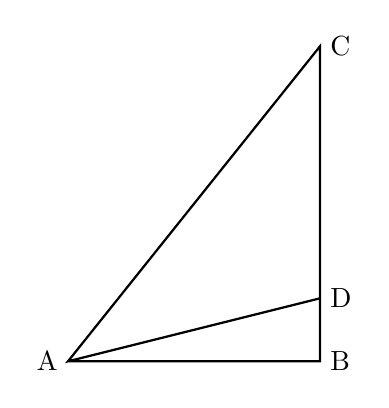
\begin{tikzpicture}[thick,x=0.8cm,y=0.8cm]
\coordinate (A) at (0,0);
\coordinate (B) at (4,0);
\coordinate (D) at (4,1);
\coordinate (C) at (4,5);
\draw (A) -- (B) -- (D) -- (A) -- (C) -- (D) ;
\path (A) node[below, left] {A} -- (B) node[below, right] {B} -- (D) node[right] {D} -- (C) node[above, right] {C};
\end{tikzpicture}
\end{document}

